\chapter{Measuring the Helicity Polarisation of the $\PW$ Boson}
\section{Introduction}
The study of \Wjets production at a hadron collider presents an important
opportunity for furthering understanding of the underlying Electroweak and
\ac{QCD} processes. In particular, since it is one of a relatively small number
of processes for which highly precise \ac{NLO} calculations have been performed,
experimental measurements can give a direct constraint on the \acp{PDF}. \Wjets
production is also of considerable interest in the context of \ac{NP} searches
where these events are often a dominant background. Finally, the neutrino in the
leptonic decay mode provides a source of ``real'' missing energy which can be
useful in the understanding of detector effects relevant to searches for
\acs{WIMP}-type particles present in \ac{SUSY} and other theories.

\section{Background}
Some theoretical background relating to \PW helicity effects has been presented
in Section~TODO. Here, the discussion will be oriented towards a more
experimental context.

For small values of \PW transverse momentum, \PtW the differential angular
cross-section for the process
$\Pp\Pp\longrightarrow\PWpm\longrightarrow\Plpm\Pgnl$ follows the Drell-Yan
distribution
\begin{equation}
\frac{dN}{d(\cos\theta)} \propto (1\mp \cos\theta)^2
\end{equation}

It is well known from straightforward helicity arguments\cite{mirkes_w_1994}that
\PW produced along the beam axis will exhibit a 100\% left-handed polarization. This
can be seen by considering the leading order partonic subprocesses
\begin{equation}
\Pup\APdown \longrightarrow \PWp \qquad\textrm{and}\qquad
\Pdown\APup\longrightarrow\PWm
\end{equation}
Firstly, note that the fraction of the proton momentum carried by the quark (as
determined by the \aclp{PDF}) is greater than that of the anti-quark. In
addition given that the \ac{LHC} is a $\Pp\Pp$ collider, valence anti-quarks are
not present. Anti-quarks must be drawn from the sea and are therefore likely to
be low momentum. Taking these two facts together, the quark is very likely to be
higher momentum than the anti-quark. By momentum conservation, it is expected
that the \PW will be produced overwhelmingly in the direction of the original
quark. Then given the \VminusA nature of the weak interaction, it is seen that
the quark must be left-handed and, by helicity conservation the \PW will be
polarised nearly 100\% left-handedly along the beam axis. A small dilution will
occur in instances where the anti-quark has by chance a larger momentum fraction
than the quark.

It is worth mentioning that the situation is not identical at the Tevatron
$\Pp\Pap$ collider. Although the \PWp also possess a 100\% left-handed
polarisation along the beamline (via similar arguments to those given above),
the \PWm are found to have a near 100\% right-handed polarisation. This is a
result of the subprocess $\APup\Pdown\longrightarrow\PWm$ where this time the
\APup carries more momentum.

In the case, where the \PW carries a significant transverse momentum \PtW, the
situation is more complex.


\begin{figure}
\centering
\subfloat[]{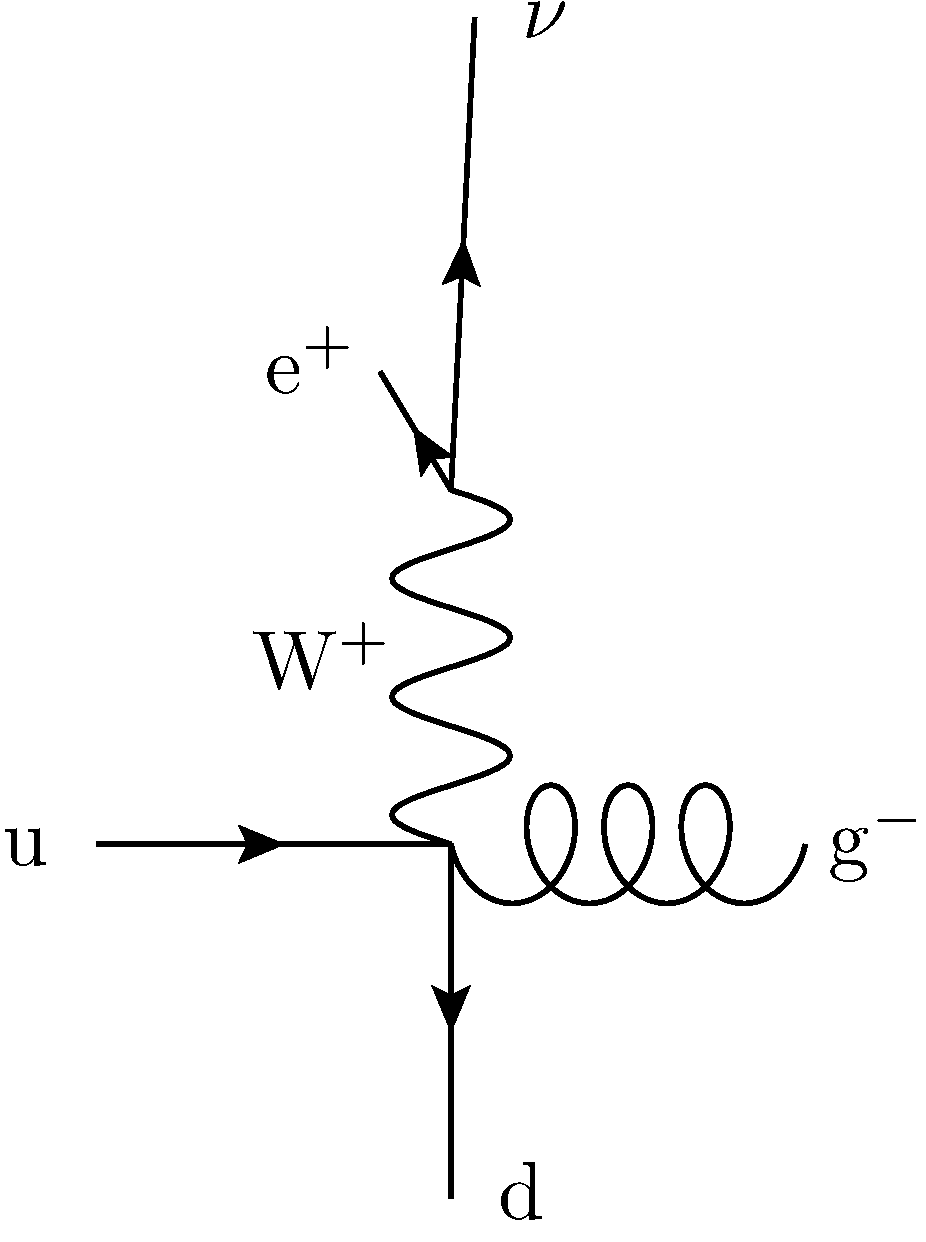
\includegraphics[width=0.3\textwidth]{fig/wpol_prod_a}}\quad
\subfloat[]{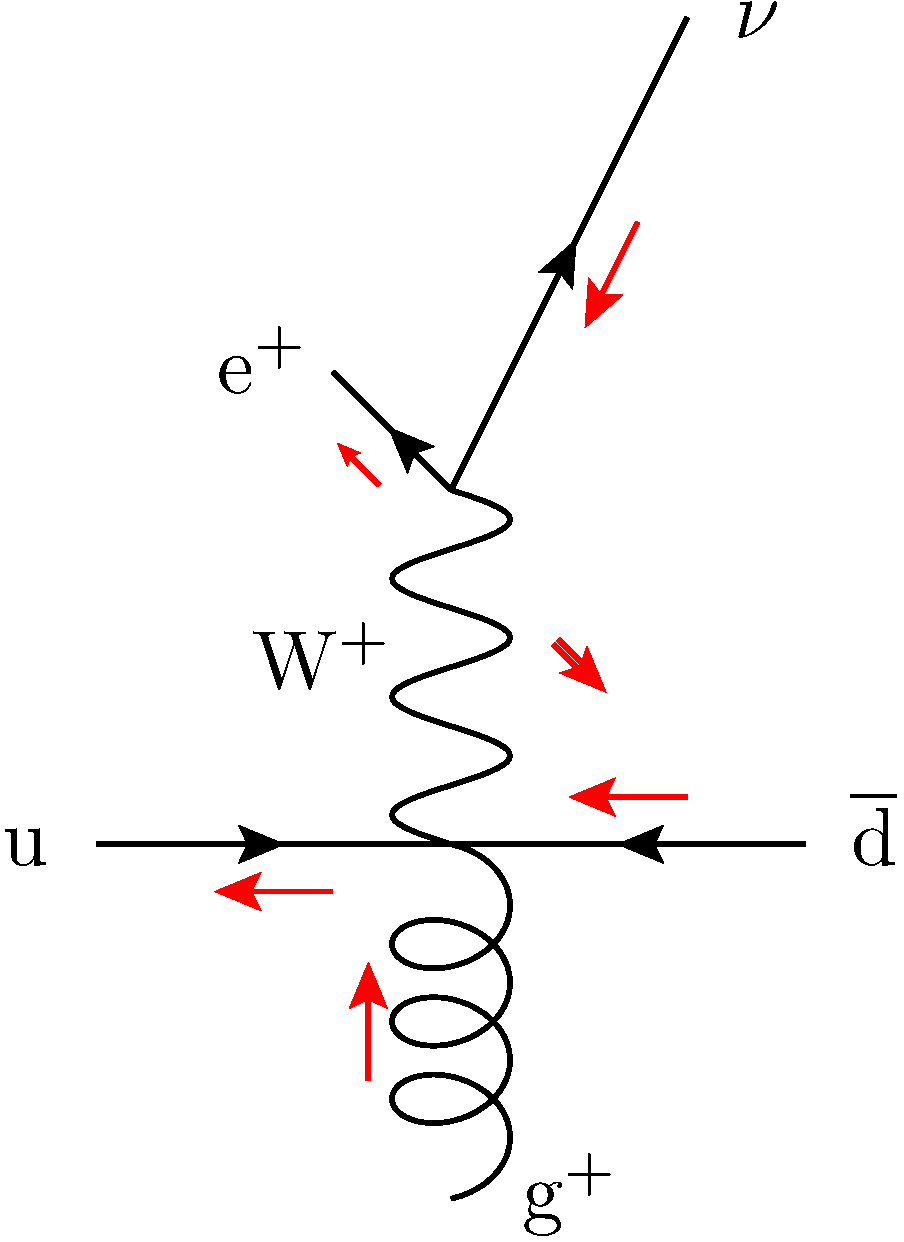
\includegraphics[width=0.3\textwidth]{fig/wpol_prod_b}}\quad
\subfloat[]{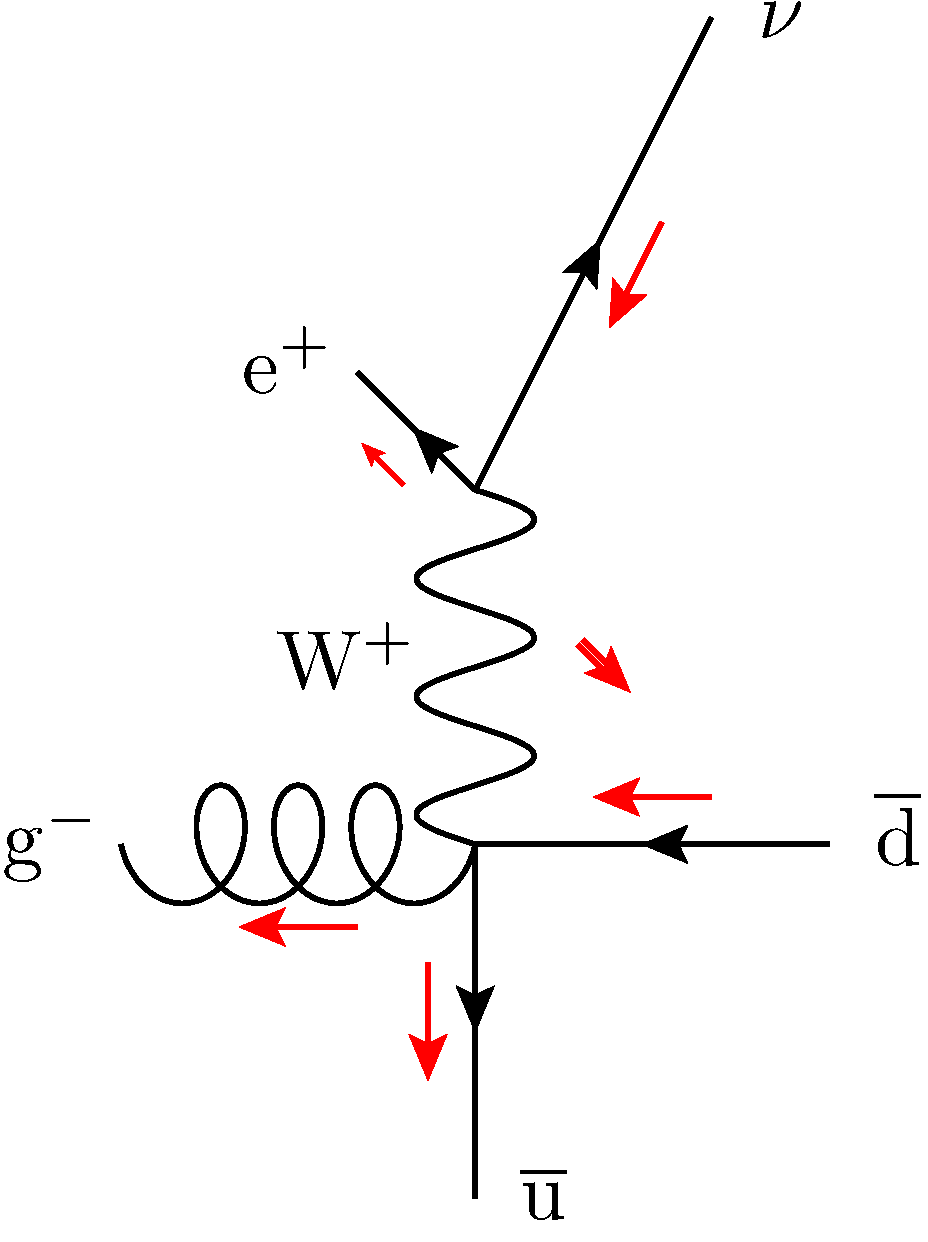
\includegraphics[width=0.3\textwidth]{fig/wpol_prod_c}}\\
\subfloat[]{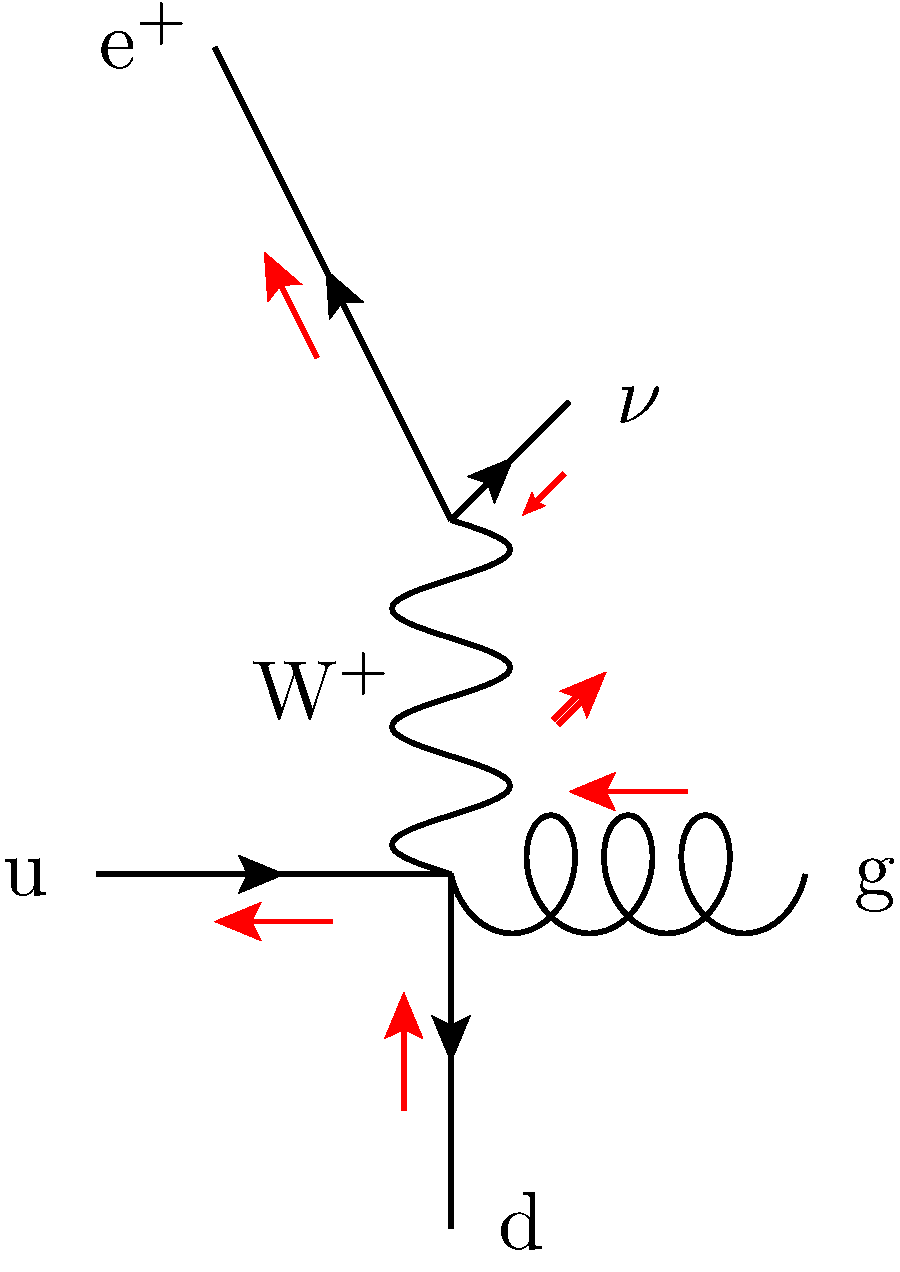
\includegraphics[width=0.3\textwidth]{fig/wpol_prod_d}}\quad
\subfloat[]{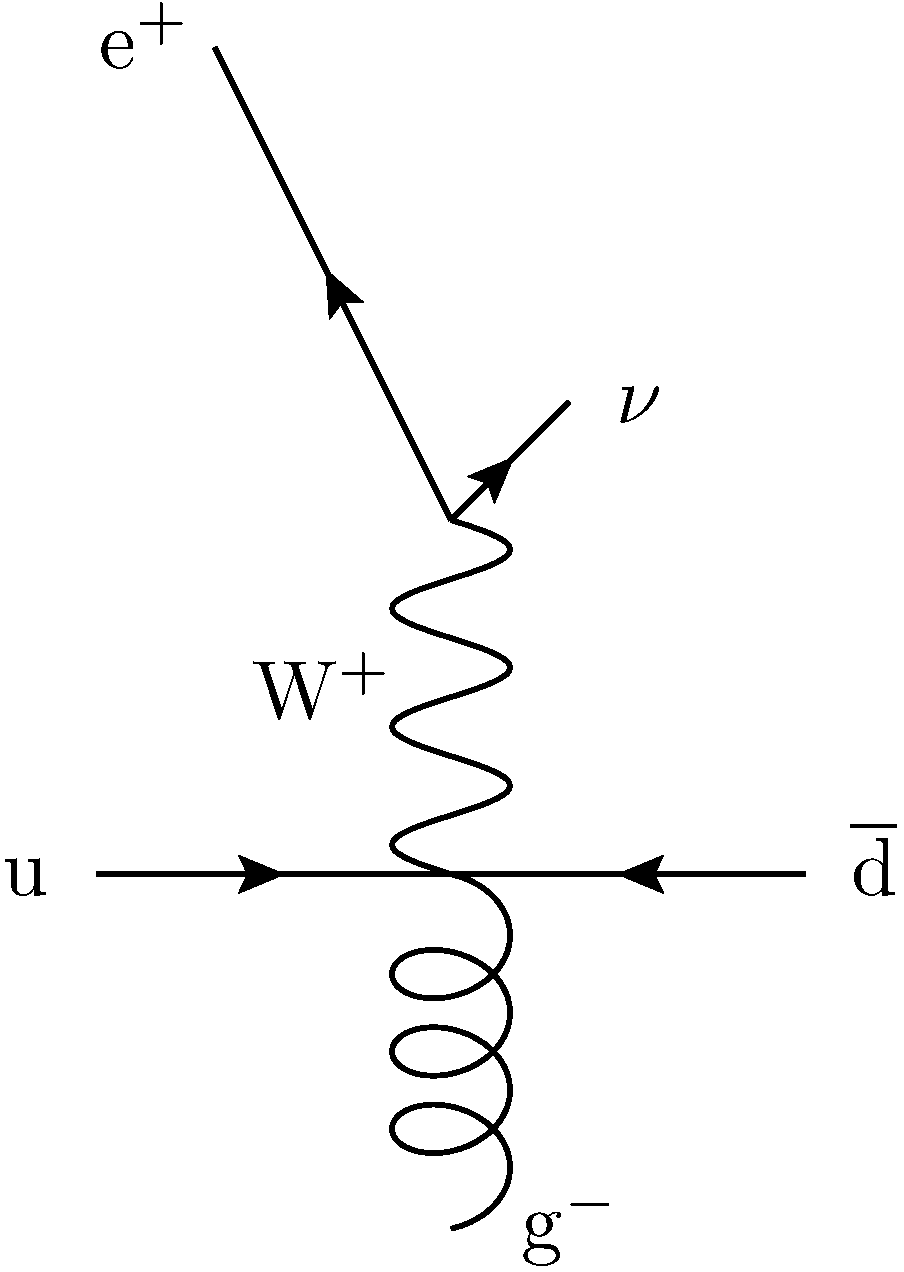
\includegraphics[width=0.3\textwidth]{fig/wpol_prod_e}}\quad
\subfloat[]{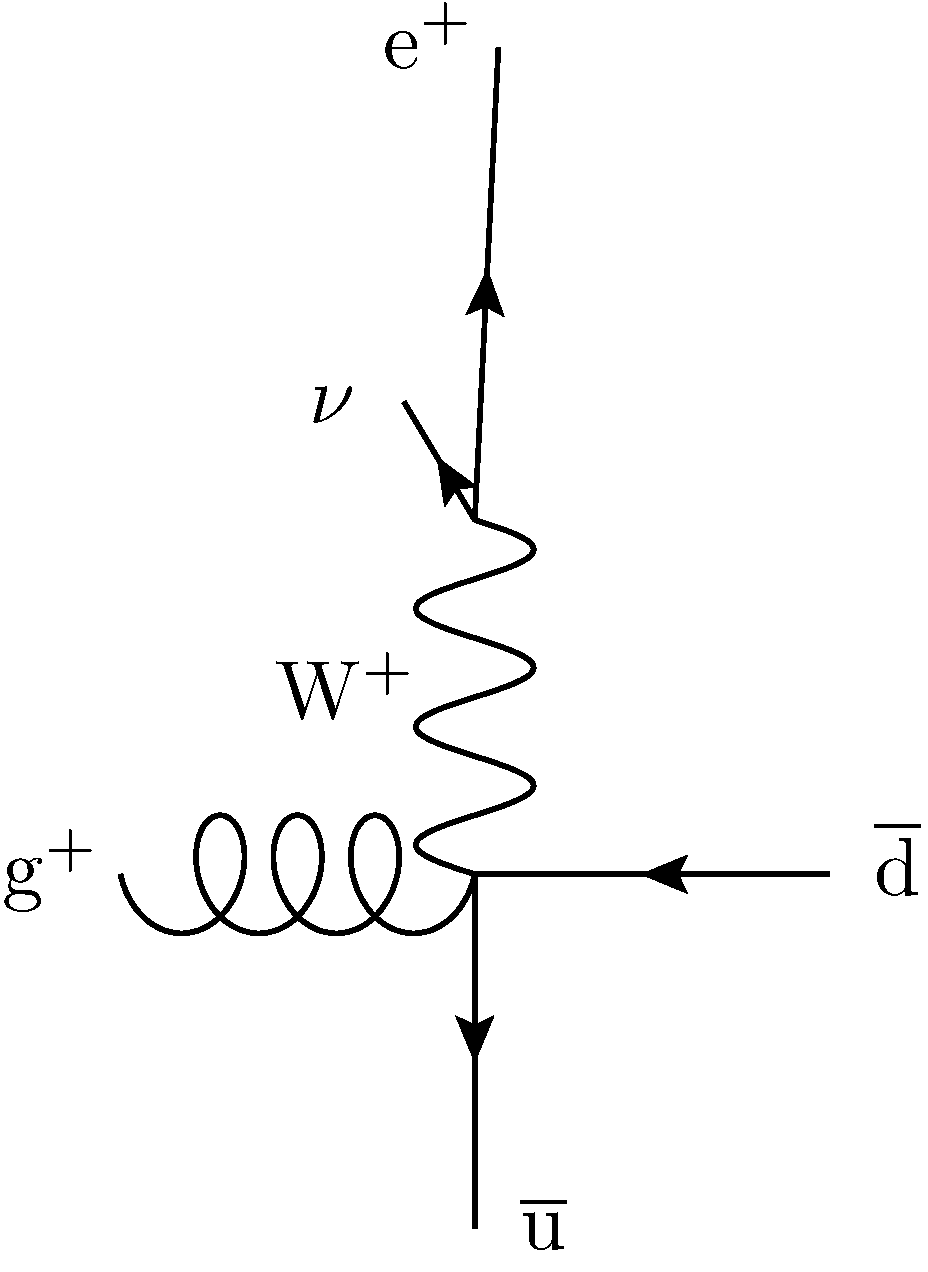
\includegraphics[width=0.3\textwidth]{fig/wpol_prod_f}}
\caption{Illustrations of $\PWplus+1$~jet production modes at the LHC. The
  $\Pgluon$ superscript indicates its helicity}
\label{fig:w1jet_modes}
\end{figure}